\vspace{-5pt}
\section{引言}
\label{sec:intro}
\vspace{-2pt}

随着空间计算的迅速发展,房间重识别(Room ReID)已成为一个关键研究领域,推动了诸如增强现实(AR)\cite{schult2023controlroom3droomgenerationusing} 和居家护理机器人 \cite{sarch2022tideetidyingnovelrooms} 等应用的进步。它在多种场景中提升用户体验方面发挥着至关重要的作用。  
例如,在 Apple Vision Pro 等设备上,精确的房间重识别能够实现虚拟与现实元素之间的平滑过渡。  
同样,在 AR 引导的博物馆导览中,准确识别用户在特定房间内的位置对于提供基于位置的内容至关重要。

\begin{figure}[ht]
    \centering
    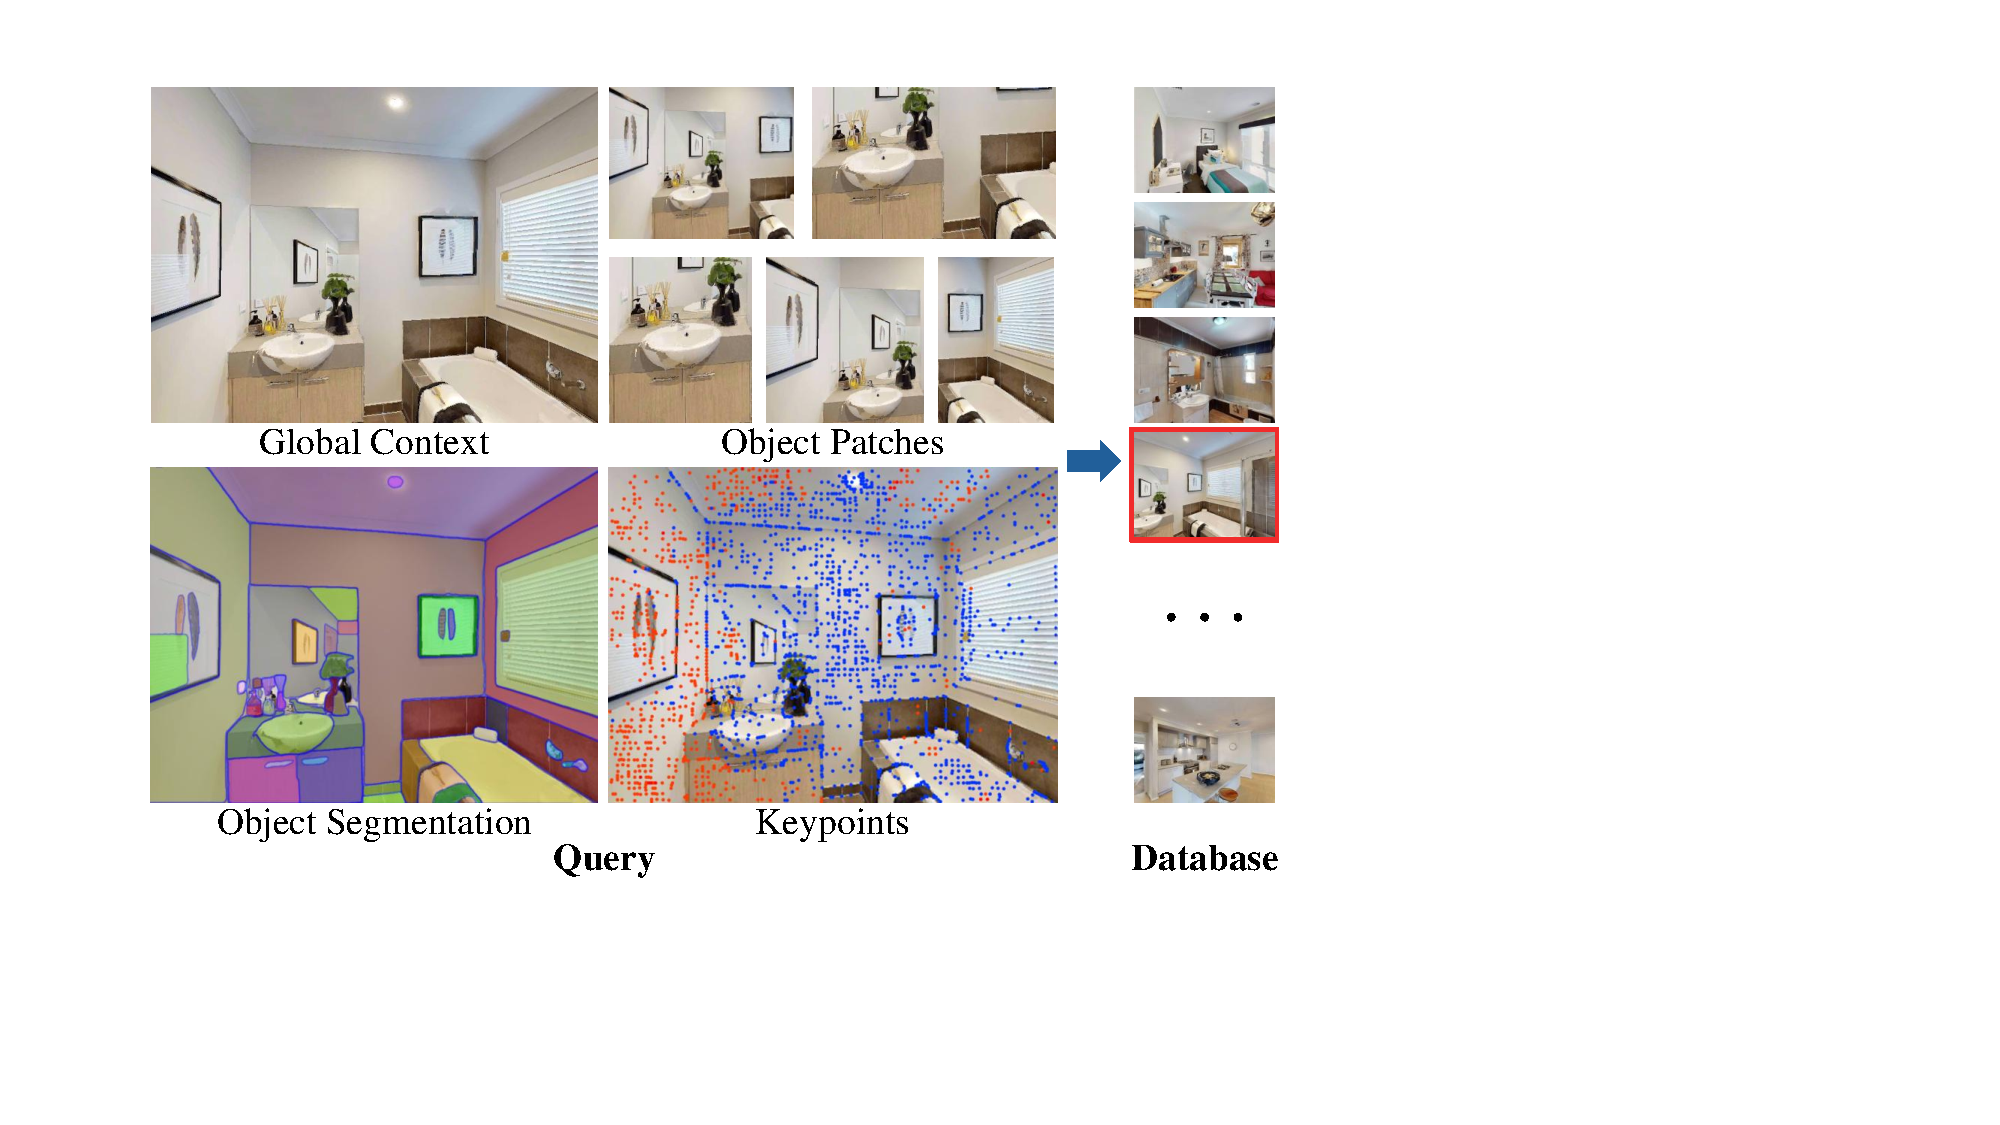
\includegraphics[width=\columnwidth]{object_information_font.pdf}
    \vspace{-20pt}
    \caption{AirRoom 利用多层次、面向对象的特征,包括全局上下文、目标区域、目标分割和关键点,执行由粗到细的房间重新识别。}
    \vspace{-20pt}
    \label{fig:example_image}
\end{figure}

与室外环境中已经成熟且表现可靠的视觉位置识别(VPR)方法不同 \cite{arandjelović2016netvladcnnarchitectureweakly, hausler2021patchnetvladmultiscalefusionlocallyglobal, keetha2023anylocuniversalvisualplace},室内房间重识别仍然是一个具有挑战性的问题。造成这一困难的主要原因在于室内场景的杂乱特性,这些场景通常密集布置着大量人造物体 \cite{xu2023clusvprefficientvisualplace}。这些密集分布的物体对现有方法构成了重大挑战,而这些方法最初是为城市风格和结构清晰的环境设计的 \cite{7339473}。因此,这些方法难以充分捕捉室内环境中复杂的细节和多样的空间布局。  
例如,像 DINO \cite{caron2021emergingpropertiesselfsupervisedvision} 和 DINOv2 \cite{oquab2024dinov2learningrobustvisual} 等基础模型能够生成捕捉整体场景特征的全局描述符。然而,在语义相似的环境中,例如布局或装饰风格相近的相邻房间,这些描述符可能难以区分细微差别 \cite{cai2022patchnetvladlearnedpatchdescriptor}。相比之下,Patch-NetVLAD \cite{hausler2021patchnetvladmultiscalefusionlocallyglobal}、AirLoc \cite{aryan2023airlocobjectbasedindoorrelocalization} 和 AnyLoc \cite{keetha2023anylocuniversalvisualplace} 等方法通过聚合局部特征来构建全局描述符,从而提升区分能力。尽管如此,在物体高度相似且重复出现的室内环境中,这些方法仍可能难以区分相似特征,从而降低在此类场景中的效果 \cite{sattler2019understandinglimitationscnnbasedabsolute}。

此外,与依赖物体类型识别以将空间分类为语义类别的房间分类方法不同 \cite{lee2017roomnetendtoendroomlayout},房间重识别的目标是在给定查询图像的基础上,从参考数据库中精确检索出同一个房间实例。  
例如,重新识别某个特定厨房需要结合全局功能上下文以及对特定物体属性的细粒度匹配。  
此外,房间重识别还需应对视角变化,因此必须具备容忍物体排列和外观部分不匹配的能力。这些需求常常导致仅基于物体分类的算法失效,因为它们缺乏准确识别唯一房间实例所需的精度 \cite{Snderhauf2015PlaceRW}。

这引出了一个重要问题:\textit{“哪些物体属性对于房间重识别是真正关键的?”}  
为了解决这个问题,我们开展了首个全面研究,探索多层次面向物体的信息及其对房间重识别的影响。  
如 \fref{fig:example_image} 所示,我们的实验表明,四种层次的面向物体信息,即全局上下文、物体图块、物体分割以及关键点,都是必不可少的。  
具体而言,我们发现每个层次在房间重识别中扮演着独特的角色。全局上下文(例如沙发与电视的组合)传达了用于将房间分类为客厅的关键语义信息。物体图块提供更精细的细节,使得可以在房间内部进行区分,例如将卧室中的床头柜与工作区的书桌区分开来。物体分割进一步细化,通过分离餐桌与周围椅子等个体物体,有助于澄清房间布局。最后,物体上的关键点(如衣柜上的把手)可通过过滤其他房间中外观相似的家具来增强房间重识别的能力。此外,集成多层次的面向物体信息还能增强对视角变化的鲁棒性。

基于上述观察,我们提出了 AirRoom——一个简单却高效的房间重识别系统(ReID),该系统由三个阶段组成:全局、局部和细粒度阶段。  
在全局阶段,使用全局特征提取器捕捉全局上下文特征,进而粗略筛选出五个功能相似的候选房间。  
在局部阶段,首先应用实例分割识别出单个物体,然后通过感受野扩展器提取物体图块。接着使用物体特征提取器提取物体及图块特征,并通过面向物体的评分机制将候选范围缩小到两个房间。  
最后,在细粒度阶段,利用特征匹配精确地识别出最终房间。

总之,我们的贡献包括:

\begin{itemize}[leftmargin=2em]
    \item 我们介绍了AirRoom,一种基于物体感知的房间重识别管道,具有两个新颖的模块:感受野扩展器和物体感知评分,充分利用多层次的面向物体的信息,克服了以往方法中的局限性。
    \item 我们精心整理了四个全面的房间重识别数据集——MPReID、HMReID、GibsonReID 和 ReplicaReID——为评估房间重识别方法提供了多样化的基准。
    \item 大量实验表明,AirRoom超越了当前的最先进技术,在显著的视角变化下仍能保持强大的可靠性和稳定的性能。
\end{itemize}
